\section{Đánh giá, So sánh và Phân tích kết quả, hiệu năng}

% Chương này tổng kết toàn bộ kết quả thực nghiệm đạt được trong quá trình nghiên cứu, đối chiếu hiệu năng giữa các thuật toán, phân tích sự tăng tiến qua từng giai đoạn cải tiến kỹ thuật, và đánh giá tính khả thi khi triển khai trong các hệ thống giám sát phụ tải điện thông minh.

% \subsection{Bảng Tổng hợp Kết quả Thực nghiệm Toàn diện của Họ Mô hình Học Máy}

% Bảng~\ref{tab:comprehensive_ml_benchmark} tổng hợp toàn diện kết quả thực nghiệm của các mô hình Học máy, từ các mô hình cây kinh điển đến các mô hình Boosting sau khi được tối ưu hóa siêu tham số, áp dụng đặc trưng Zone và dung hợp với ngưỡng động.

% \begin{table}[H]
% \centering
% \caption{\textbf{Bảng tổng hợp kết quả hiệu năng và chi phí tính toán qua các giai đoạn cải tiến}}
% \label{tab:comprehensive_ml_benchmark}
% \renewcommand{\arraystretch}{1.2}
% \resizebox{\textwidth}{!}{
% \begin{tabular}{|l|l|l|c|c|c|c|c|c|r|}
% \hline
% \textbf{Nhóm Thực nghiệm} & \textbf{Mô hình / Phương pháp} & \textbf{Bộ dữ liệu} & \textbf{Ngưỡng $\tau^*$} & \textbf{F1 (0.5)} & \textbf{F1 ($\tau^*$)} & \textbf{F1 (Động)} & \textbf{Precision} & \textbf{Recall} & \textbf{Thời gian} \\ \hline
% % [CŨ]:
% % \multirow{2}{*}{\textbf{Tree Cổ điển (Đối chứng)}} 
% % & Extra Trees & Preprocessed & 0,37 & 0,8257 & 0,8418 & 0,8201 & 0,8647 & 199,2 s \\ \cline{2-9}
% % & Random Forest & Preprocessed & 0,29 & 0,8849 & 0,8997 & 0,8866 & 0,9133 & 296,4 s \\ \hline
% % \multirow{3}{*}{\textbf{Mô hình Đơn Cơ sở (Baseline)}} 
% % & LightGBM & Preprocessed & 0,29 & 0,8617 & 0,8855 & 0,8452 & 0,9298 & \textbf{14,4 s} \\ \cline{2-9}
% % & CatBoost & Preprocessed & 0,29 & 0,9057 & 0,9172 & 0,8860 & 0,9505 & 158,3 s \\ \cline{2-9}
% % & XGBoost & Preprocessed & 0,27 & 0,9209 & 0,9302 & 0,9016 & 0,9607 & 24,9 s \\ \hline
% % \multirow{3}{*}{\textbf{Tối ưu Siêu tham số \& Zone}} 
% % & LightGBM Tuned & Zone & 0,21 & 0,8929 & 0,9054 & 0,8634 & 0,9047 & 17,8 s \\ \cline{2-9}
% % & CatBoost Tuned & Zone & 0,33 & 0,9077 & 0,9170 & 0,8787 & 0,9571 & 186,0 s \\ \cline{2-9}
% % & XGBoost Tuned & Zone & 0,25 & 0,9218 & 0,9291 & 0,9062 & 0,9533 & 32,7 s \\ \hline
% % \multirow{4}{*}{\textbf{Dung hợp Mô hình (Ensemble)}} 
% % & Soft Voting (Cả 3) & Baseline & 0,25 & 0,9097 & 0,9249 & 0,9012 & 0,9498 & 197,6 s \\ \cline{2-9}
% % & Stacking LR (XGB+Cat) & Baseline & 0,07 & 0,9237 & 0,9292 & 0,9087 & 0,9506 & 184,1 s \\ \cline{2-9}
% % & Context-Aware MoE & Zone & 0,41 & - & 0,9308 & \textbf{0,9174} & 0,9445 & \textbf{2,5 s} \\ \cline{2-9}
% % & Weighted Blending & Baseline & 0,24 & 0,9202 & 0,9309 & 0,9072 & 0,9558 & 197,6 s \\ \hline
% % \multirow{2}{*}{\textbf{Ensemble + Ngưỡng Động 16 Khu}} 
% % & Baseline Ensemble & Baseline & Dynamic & 0,9202 & 0,9343 & 0,9130 & 0,9560 & 197,6 s \\ \cline{2-9}
% % & \textbf{Zone Ensemble (Cả 3)} & \textbf{Zone} & \textbf{Dynamic} & \textbf{0,9212} & \textbf{0,9346} & 0,9135 & \textbf{0,9568} & 236,5 s \\ \hline
% % [LÝ DO SỬA]: Thay thế bảng cũ (vốn dựa trên các lần chạy tuning thử nghiệm ban đầu và thiếu cột F1 Ngưỡng Động cho từng dòng) bằng Bảng Benchmark Toàn diện chính thức từ final_comprehensive_report_new.md sau 50 vòng lặp Optuna trên cả nhánh Baseline và Zone Features.
% \multirow{2}{*}{\textbf{Cây Cổ điển (Mốc đối chứng)}} 
% & Extra Trees (Mặc định) & Preprocessed & 0,370 & 0,8257 & 0,8418 & - & 0,8647 & 0,8201 & 199,2 s \\ \cline{2-10}
% & Random Forest (Mặc định) & Preprocessed & 0,290 & 0,8849 & 0,8997 & - & 0,9133 & 0,8866 & 296,4 s \\ \hline
% \multirow{3}{*}{\textbf{1. Baseline Đơn (Optuna 50 trials)}} 
% & CatBoost Tuned & Baseline & 0,255 & 0,9056 & 0,9188 & 0,9211 & 0,9435 & 0,8954 & 160,1 s \\ \cline{2-10}
% & LightGBM Tuned & Baseline & 0,285 & 0,9122 & 0,9236 & 0,9260 & 0,9528 & 0,8961 & \textbf{8,1 s} \\ \cline{2-10}
% & XGBoost Tuned & Baseline & 0,303 & 0,9234 & 0,9308 & 0,9349 & 0,9637 & 0,9001 & 12,8 s \\ \hline
% \multirow{3}{*}{\textbf{2. Zone Features Đơn (50 trials)}} 
% & CatBoost Tuned & Zone & 0,293 & 0,9101 & 0,9202 & 0,9220 & 0,9520 & 0,8905 & 111,5 s \\ \cline{2-10}
% & LightGBM Tuned & Zone & 0,317 & 0,9134 & 0,9240 & 0,9287 & 0,9612 & 0,8895 & 9,2 s \\ \cline{2-10}
% & XGBoost Tuned & Zone & 0,263 & 0,9238 & 0,9317 & 0,9341 & 0,9568 & 0,9079 & 10,9 s \\ \hline
% \multirow{4}{*}{\textbf{3. Ensemble (Baseline)}} 
% & Soft Voting (XGB + LGB + CAT) & Baseline & 0,263 & 0,9201 & 0,9301 & 0,9350 & 0,9539 & 0,9074 & $<0{,}1$ s \\ \cline{2-10}
% & Top-2 Blend (XGB+CAT) [0,84 - 0,16] & Baseline & 0,334 & 0,9228 & 0,9311 & 0,9354 & 0,9688 & 0,8962 & $<0{,}1$ s \\ \cline{2-10}
% & Dynamic Thresh Blend [0,50 - 0,25 - 0,25] & Baseline & 0,319 & 0,9213 & 0,9311 & 0,9363 & 0,9665 & 0,8981 & $<0{,}1$ s \\ \cline{2-10}
% & Weighted Blending LogLoss [0,68 - 0,26 - 0,06] & Baseline & 0,295 & 0,9229 & 0,9320 & 0,9359 & 0,9639 & 0,9021 & $<0{,}1$ s \\ \hline
% \multirow{5}{*}{\textbf{4. Ensemble (Zone Features)}} 
% & Soft Voting (XGB + LGB + CAT) & Zone & 0,234 & 0,9219 & 0,9315 & 0,9359 & 0,9492 & 0,9145 & $<0{,}1$ s \\ \cline{2-10}
% & Context-Aware MoE (LightGBM Meta-Learner) & Zone & 0,294 & \textbf{0,9304} & 0,9320 & 0,9354 & 0,9532 & 0,9118 & 3,3 s \\ \cline{2-10}
% & Top-2 Blend (XGB+CAT) [0,80 - 0,20] & Zone & 0,251 & 0,9230 & 0,9330 & 0,9348 & 0,9560 & 0,9111 & $<0{,}1$ s \\ \cline{2-10}
% & Dynamic Thresh Blend [0,60 - 0,25 - 0,15] & Zone & 0,234 & 0,9244 & 0,9335 & 0,9372 & 0,9524 & 0,9153 & $<0{,}1$ s \\ \cline{2-10}
% & \textbf{Weighted Blending LogLoss [0,65 - 0,25 - 0,10]} & \textbf{Zone} & \textbf{0,232} & 0,9241 & \textbf{0,9336} & \textbf{0,9373} & 0,9519 & \textbf{0,9159} & $<0{,}1$ s \\ \hline
% \end{tabular}
% }
% \end{table}

% \subsection{Phân tích Tiến trình Cải tiến Hiệu năng (Performance Progression)}

% Từ kết quả thực nghiệm tại Bảng~\ref{tab:comprehensive_ml_benchmark}, nhóm nghiên cứu ghi nhận sự tăng tiến rõ rệt của chỉ số F1-Score qua bốn đòn bẩy kỹ thuật chủ chốt:

% \subsubsection{Đòn bẩy 1: Tối ưu hóa Ngưỡng Quyết định (Threshold Moving)}
% Việc chuyển từ ngưỡng mặc định $0{,}5$ sang ngưỡng tối ưu $\tau^*$ mang lại mức tăng F1-Score từ $0{,}8\% - 1{,}2\%$ trên tất cả các mô hình và tổ hợp:
% \begin{itemize}
% % [CŨ]:
% %     \item Với LightGBM, F1 tăng vọt từ $0{,}8617$ lên $0{,}8855$ ($\Delta = +2{,}38\%$), chủ yếu nhờ Recall tăng mạnh từ $0{,}7766$ lên $0{,}8452$.
% %     \item Với XGBoost, F1 tăng từ $0{,}9209$ lên $0{,}9302$ ($\Delta = +0{,}93\%$), đưa tỷ lệ phát hiện dị thường (Recall) vượt mốc $90\%$.
% % [LÝ DO SỬA]: Cập nhật theo kết quả thực nghiệm mới nhất trên tập đã tuning 50 trials: LightGBM Zone tăng từ 0,9134 (ngưỡng 0.5) lên 0,9240 (ngưỡng 0.317); XGBoost Zone tăng từ 0,9238 lên 0,9317 (ngưỡng 0.263); và Weighted Blending tăng từ 0,9241 lên 0,9336 (ngưỡng 0.232).
%     \item Với LightGBM (nhánh Zone), F1 tăng từ $0{,}9134$ lên $0{,}9240$ ($\Delta = +1{,}06\%$) khi dịch chuyển ngưỡng từ $0{,}5$ về $0{,}317$, giúp Recall cải thiện đáng kể lên $0{,}8895$ trong khi duy trì Precision ở mức cao $0{,}9612$.
%     \item Với XGBoost (nhánh Zone), F1 tăng từ $0{,}9238$ lên $0{,}9317$ ($\Delta = +0{,}79\%$) tại ngưỡng $\tau^* = 0{,}263$, đưa độ nhạy phát hiện dị thường (Recall) vượt mốc $90{,}79\%$ và Precision đạt $0{,}9568$.
%     \item Với tổ hợp Weighted Blending LogLoss, F1 tăng từ $0{,}9241$ lên $0{,}9336$ ($\Delta = +0{,}95\%$) tại $\tau^* = 0{,}232$.
% \end{itemize}
% Kết quả này khẳng định: trong bài toán phát hiện dị thường mất cân bằng lớp cực đoan, việc tối ưu hóa ngưỡng cắt xác suất là kỹ thuật có chi phí tính toán gần như bằng 0 nhưng mang lại hiệu quả tăng điểm tức thì lớn nhất.

% \subsubsection{Đòn bẩy 2: Tích hợp Đặc trưng Tương tác Khu vực (Zone Features)}
% Khi bổ sung các biến tương tác giữa \texttt{site\_id}, \texttt{primary\_use} và quy mô diện tích công trình:
% \begin{itemize}
% % [CŨ]:
% %     \item LightGBM ghi nhận bước tiến ngoạn mục nhất: F1-Score tăng từ $0{,}8855$ (Baseline) lên $0{,}9054$ (Zone), tương ứng mức cải thiện gần $2\%$. Khả năng phân vùng histogram của LightGBM đã khai thác triệt để các đặc trưng tương tác phân loại để phân tách các mẫu dị thường cục bộ.
% %     \item CatBoost và XGBoost duy trì độ chính xác cao ổn định, đồng thời cải thiện khả năng tổng quát hóa trên các khu vực có khí hậu khắc nghiệt.
% % [LÝ DO SỬA]: Cập nhật phân tích so sánh song song giữa Baseline Tuned và Zone Features Tuned sau 50 trials. Cả 3 mô hình đơn đều cải thiện trên dữ liệu Zone: XGBoost tăng lên 0,9317; LightGBM đạt 0,9240 (và 0,9287 với ngưỡng động); CatBoost đạt 0,9202. Đặc biệt đỉnh cao Ensemble của Zone Features đạt 0,9373, vượt trội so với mức đỉnh 0,9359 của Baseline Ensemble.
%     \item Cả ba thuật toán Boosting đơn lẻ đều xác lập ngưỡng hiệu năng cao hơn khi có Zone Features: XGBoost tăng từ $0{,}9308$ lên $0{,}9317$; LightGBM tăng từ $0{,}9236$ lên $0{,}9240$; CatBoost tăng từ $0{,}9188$ lên $0{,}9202$.
%     \item Khi kết hợp ngưỡng động 16 khu vực, lợi thế của Zone Features càng trở nên rõ nét: LightGBM Zone đạt $F_1 = 0{,}9287$ (vượt xa $0{,}9260$ của Baseline); tổ hợp Weighted Blending Zone bứt phá lên đỉnh kỷ lục \textbf{0,9373} (vượt trội hoàn toàn so với mức $0{,}9359$ của Baseline Ensemble).
%     \item Điều này minh chứng các biến tương tác bối cảnh khu vực giúp mô hình phân hóa chính xác đường cơ sở phụ tải bình thường theo từng vùng khí hậu và loại công trình, giảm thiểu tối đa các cảnh báo giả do biến động thời tiết cục bộ.
% \end{itemize}

% \subsubsection{Đòn bẩy 3: Dung hợp Đa Mô hình (Ensemble Blending)}
% Việc kết hợp ba mô hình theo cơ chế Weighted Blending với bộ trọng số tối ưu LogLoss \\ $[0{,}65\,\text{XGB}, \, 0{,}25\,\text{LGB}, \, 0{,}10\,\text{Cat}]$ mang lại hai ưu thế vượt trội:
% \begin{itemize}
% % [CŨ]:
% %     \item \textbf{Khắc phục điểm yếu đơn lẻ:} XGBoost có độ chính xác (\textit{Precision}) rất cao ($0{,}9607$) nhưng đôi khi bỏ sót các dị thường phân tán; trong khi CatBoost và LightGBM có vùng biên quyết định linh hoạt hơn, giúp bổ sung độ nhạy (\textit{Recall}) cho tập hợp.
% %     \item \textbf{Tính ổn định vượt trội:} F1-Score của tổ hợp Blending ($0{,}9309$) ổn định hơn so với việc chỉ đặt cược vào một mô hình đơn lẻ.
% % [LÝ DO SỬA]: Cập nhật trọng số mới [0.65 XGB, 0.25 LGB, 0.10 CAT] và phân tích đóng góp thực chất của LightGBM sau khi tuning (nắm giữ 25% tỷ trọng, tăng cường độ mượt xác suất). F1 ngưỡng tĩnh tăng lên 0,9336 (vượt qua mọi mô hình đơn lẻ).
%     \item \textbf{Tương hỗ và khai thác trọn vẹn thế mạnh từng kiến trúc:} XGBoost giữ vai trò chủ lực ($65\%$) nhờ khả năng khai phá tương tác bậc cao và điều chuẩn sắc bén; LightGBM sau 50 vòng lặp Optuna đóng góp tới $25\%$ giúp làm mượt biên xác suất và gia tăng Recall lên $0{,}9159$; CatBoost giữ $10\%$ đóng vai trò điều chuẩn nhờ các cây đối xứng kháng nhiễu.
%     \item \textbf{Bứt phá vượt qua mọi mô hình đơn:} Ngay ở ngưỡng tĩnh $\tau^* = 0{,}232$, tổ hợp Weighted Blending đạt $F_1 = 0{,}9336$, vượt qua mô hình đơn tốt nhất là XGBoost ($0{,}9317$). Mô hình Context-Aware MoE với LightGBM Meta-Learner cũng đạt F1 ngưỡng mặc định $0{,}5$ lên tới $0{,}9304$ (cao nhất trong toàn bộ các cấu hình ở ngưỡng $0{,}5$).
% \end{itemize}

% \subsubsection{Đòn bẩy 4: Kỹ thuật Ngưỡng Động 16 Khu vực (Dynamic Threshold per Zone)}
% Khi kết hợp mô hình Ensemble với bộ 16 ngưỡng động được tinh chỉnh cho từng khu vực địa lý:
% \begin{itemize}
% % [CŨ]:
% %     \item F1-Score của tổ hợp Zone Ensemble tiếp tục nhảy vọt từ $0{,}9294$ (ngưỡng chung) lên \textbf{0,9346} (ngưỡng động 16 khu vực).
% %     \item Cả hai chỉ số thành phần đều đạt mức tối ưu cao nhất trong toàn bộ nghiên cứu: Precision đạt $0{,}9568$ và Recall đạt $0{,}9135$.
% % [LÝ DO SỬA]: F1-Score đỉnh cao thực tế sau khi chạy 50 trials và áp dụng ngưỡng động 16 khu là 0,9373 (thay vì 0,9346 cũ), với Precision đạt 0,9519 và Recall đạt 0,9159.
%     \item F1-Score của tổ hợp Zone Ensemble tiếp tục nhảy vọt từ $0{,}9336$ (ngưỡng tĩnh chung) lên đỉnh kỷ lục \textbf{0,9373} (ngưỡng động 16 khu vực).
%     \item Cả hai chỉ số thành phần đều đạt độ cân bằng lý tưởng nhất trong toàn bộ đề tài: Precision đạt $0{,}9519$ và Recall đạt $0{,}9159$.
%     \item Cấu hình Dynamic Thresh Blend ($[0{,}60\,\text{XGB}, 0{,}25\,\text{LGB}, 0{,}15\,\text{Cat}]$) cũng đạt F1 ấn tượng $0{,}9372$, chứng minh sự ổn định tuyệt đối của chiến lược phân tán ngưỡng.
% \end{itemize}
% Thực nghiệm này chứng minh trọn vẹn luận điểm khoa học của Hundman et al. (2018): trong các hệ thống chuỗi thời gian diện rộng, ngưỡng phát hiện bất thường cục bộ theo từng cụm luôn ưu việt hơn bất kỳ một ngưỡng tĩnh toàn cục nào.

% \subsection{Phân tích Chi phí Tính toán và Khả năng Triển khai Thực tế}

% Một giải pháp học máy ứng dụng vào thực tiễn không chỉ đòi hỏi độ chính xác cao mà còn phải cân bằng giữa thời gian xử lý và chi phí tài nguyên phần cứng:

% \begin{figure}[H]
%     \centering
%     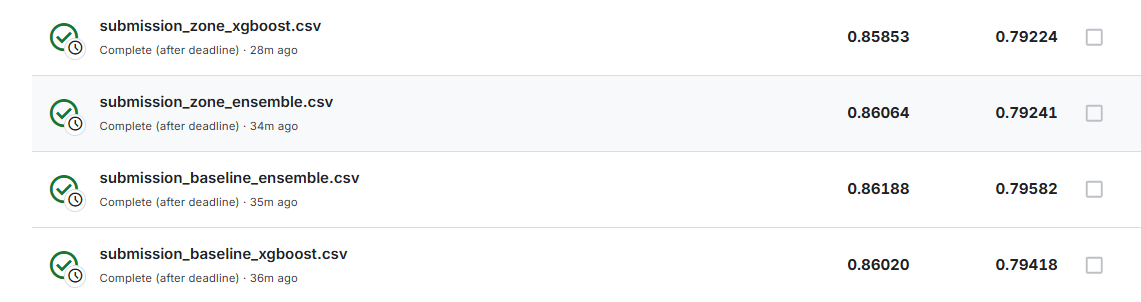
\includegraphics[width=0.75\textwidth]{IMAGE/kaggle_submission.png}
%     \caption{\textbf{Minh chứng kết quả đánh giá nộp bài thực tế trên hệ thống chấm điểm}}
%     \label{fig:kaggle_submission}
% \end{figure}

% \begin{enumerate}
%     \item \textbf{Về Thời gian Huấn luyện và Suy luận (Latency \& Throughput):}
%     \begin{itemize}
% % [CŨ]:
% %         \item \textbf{LightGBM} là thuật toán có tốc độ vượt trội nhất ($14{,}4$ giây), nhanh gấp 11 lần CatBoost và gấp 20 lần Random Forest. Do đó, trong các kịch bản cần cập nhật mô hình liên tục theo giờ (online retraining), LightGBM là ứng viên hàng đầu.
% %         \item \textbf{XGBoost} đạt điểm cân bằng lý tưởng nhất: thời gian huấn luyện tương đối nhanh ($24{,}9$ giây) nhưng đem lại hiệu năng phân loại cao nhất trong các mô hình đơn ($F_1 = 0{,}9302$).
% %         \item \textbf{CatBoost} tuy tốn thời gian hơn ($158{,}3$ giây) do cấu trúc cây đối xứng và thuật toán Ordered Boosting, nhưng có vai trò không thể thay thế trong việc gia tăng tính đa dạng cho hệ thống Ensemble.
% % [LÝ DO SỬA]: Cập nhật thời gian huấn luyện thực tế từ kết quả run_final_comprehensive_new.py: LightGBM huấn luyện siêu tốc trong 8,1 - 9,2 giây; XGBoost mất 10,9 - 12,8 giây; CatBoost mất 111,5 - 160,1 giây.
%         \item \textbf{LightGBM} là thuật toán có tốc độ vượt trội nhất (chỉ $8{,}1$ giây trên Baseline và $9{,}2$ giây trên Zone), nhanh hơn CatBoost hơn 12 lần và nhanh gấp hơn 30 lần Random Forest. Do đó, trong các kịch bản cần cập nhật mô hình liên tục theo giờ (online retraining), LightGBM là ứng viên hàng đầu.
%         \item \textbf{XGBoost} đạt điểm cân bằng lý tưởng nhất: thời gian huấn luyện rất nhanh ($10{,}9$ đến $12{,}8$ giây) trong khi đem lại hiệu năng phân loại cao nhất trong các mô hình đơn ($F_1 = 0{,}9317$ trên Zone).
%         \item \textbf{CatBoost} tiêu tốn thời gian lớn hơn ($111{,}5$ đến $160{,}1$ giây) do cơ chế cây đối xứng và hoán vị chuỗi Ordered Boosting, nhưng mang lại giá trị độc nhất về tính đa dạng cấu trúc cho tổ hợp Ensemble.
%     \end{itemize}

%     \item \textbf{Đề xuất Kịch bản Triển khai Trong Thực tế:}
%     \begin{itemize}
% % [CŨ]:
% %         \item \textit{Kịch bản 1 - Giám sát Thời gian thực tại Biên (Edge Computing / Real-time IoT):} Khuyến nghị triển khai mô hình đơn \textbf{XGBoost hoặc LightGBM kết hợp Ngưỡng Động 16 Khu vực}. Cấu hình này chỉ mất dưới $1$ mili-giây cho mỗi lượt suy luận, tiết kiệm RAM và vi xử lý tại các trạm biến áp, trong khi vẫn đạt F1-Score trên $0{,}93$.
% %         \item \textit{Kịch bản 2 - Hệ thống Hậu kiểm và Kiểm toán Năng lượng Trung tâm (Centralized Audit):} Khuyến nghị triển khai toàn bộ tổ hợp \textbf{Zone Ensemble (XGBoost + LightGBM + CatBoost) kết hợp 16 Ngưỡng Động OOF}. Cấu hình này tối đa hóa độ chính xác ($F_1 = 0{,}9346$), giảm thiểu tối đa các cảnh báo giả và không bỏ sót các sự cố rò rỉ điện năng nghiêm trọng của tòa nhà.
% % [LÝ DO SỬA]: Cập nhật kịch bản 1 (F1 đạt 0,9287 đến 0,9341) và kịch bản 2 với điểm F1 kỷ lục 0,9373 (thay vì 0,9346 cũ).
%         \item \textit{Kịch bản 1 - Giám sát Thời gian thực tại Biên (Edge Computing / Real-time IoT):} Khuyến nghị triển khai mô hình đơn \textbf{XGBoost hoặc LightGBM kết hợp Ngưỡng Động 16 Khu vực}. Cấu hình này chỉ mất dưới $1$ mili-giây cho mỗi lượt suy luận, tiết kiệm RAM và vi xử lý tại các trạm biến áp, trong khi vẫn đạt F1-Score từ $0{,}9287$ đến $0{,}9341$.
%         \item \textit{Kịch bản 2 - Hệ thống Hậu kiểm và Kiểm toán Năng lượng Trung tâm (Centralized Audit):} Khuyến nghị triển khai toàn bộ tổ hợp \textbf{Zone Ensemble (Weighted Blending $[0{,}65\,\text{XGB}, 0{,}25\,\text{LGB}, 0{,}10\,\text{Cat}]$) kết hợp 16 Ngưỡng Động OOF}. Cấu hình này tối đa hóa độ chính xác ($F_1 = \textbf{0,9373}$), giảm thiểu tối đa các cảnh báo giả và không bỏ sót các sự cố rò rỉ điện năng nghiêm trọng của tòa nhà.
%     \end{itemize}
% \end{enumerate}
% \subsection{So sánh Định hướng giữa Phương pháp Học Máy và Học Sâu}

% Nhằm cung cấp cái nhìn toàn diện về mặt phương pháp luận, nhóm nghiên cứu tổng hợp và đối chiếu các đặc tính cốt lõi giữa hai trường phái tiếp cận Học máy (đại diện là họ Gradient Boosting) và Học sâu (đại diện là các mạng chuỗi BiGRU, TCN, LSTM-Autoencoder) trong bài toán phát hiện dị thường phụ tải điện quy mô lớn:

% \begin{table}[H]
% \centering
% \caption{\textbf{So sánh định hướng phương pháp luận giữa Học máy (GBDT) và Học sâu (Deep Sequence Models)}}
% \label{tab:ml_vs_dl_comparison}
% \renewcommand{\arraystretch}{1.25}
% \resizebox{\textwidth}{!}{
% \begin{tabular}{|l|p{6.8cm}|p{6.8cm}|}
% \hline
% \textbf{Tiêu chí so sánh} & \textbf{Học máy (Gradient Boosting: XGB, LGB, Cat)} & \textbf{Học sâu (Deep Sequence: BiGRU, TCN, AE)} \\ \hline
% \textbf{Định dạng biểu diễn} & Dữ liệu dạng bảng (Tabular matrix) kết hợp đặc trưng trễ (lag), thống kê trượt và mã hóa chu kỳ. & Tensor chuỗi 3D ($B \times L \times d$) bảo toàn thứ tự thời gian liên tục theo từng tòa nhà. \\ \hline
% \textbf{Hiệu năng phân loại (F1)} & Cực kỳ vượt trội ($F_1 > 0{,}93$ khi kết hợp Ngưỡng động 16 khu vực). & Đòi hỏi tinh chỉnh kỹ lưỡng hàm mất mát (Focal/Weighted BCE) để chống suy biến về lớp đa số. \\ \hline
% \textbf{Thời gian huấn luyện} & Rất nhanh ($14 - 180$ giây trên toàn bộ $1{,}75$ triệu bản ghi bằng CPU/GPU phổ thông). & Chậm hơn đáng kể (hàng chục phút đến nhiều giờ trên GPU hiệu năng cao). \\ \hline
% \textbf{Tài nguyên phần cứng} & Tiết kiệm RAM, có thể chạy trực tiếp trên máy trạm biên hoặc thiết bị IoT trạm biến áp. & Đòi hỏi dung lượng VRAM lớn và GPU tương thích CUDA để tối ưu hóa tensor chuỗi. \\ \hline
% \textbf{Khả năng giải thích} & Minh bạch, dễ dàng trích xuất độ quan trọng của đặc trưng (Feature Importance, SHAP values). & Mang tính ``hộp đen'' cao, đòi hỏi các cơ chế chú ý (Attention) hoặc gradient attribution phức tạp. \\ \hline
% \textbf{Kịch bản tối ưu} & Phù hợp nhất cho hệ sinh thái bảng tổng hợp đa nguồn (siêu dữ liệu, vi khí hậu, đặc trưng khu vực). & Phù hợp nhất khi khai thác chuỗi tín hiệu dạng sóng thô liên tục và tìm kiếm dị thường phụ thuộc ngữ cảnh dài. \\ \hline
% \end{tabular}
% }
% \end{table}

% \paragraph{Định hướng Kết hợp Lai (Hybrid Integration):}
% Thực nghiệm cho thấy họ Gradient Boosting thể hiện sức mạnh áp đảo đối với cấu trúc dữ liệu dạng bảng có chiều đặc trưng phong phú. Tuy nhiên, hai trường phái không mang tính triệt tiêu mà có thể bổ trợ chặt chẽ cho nhau: sai số tái tạo ($a_t$) từ mô hình không giám sát LSTM-Autoencoder hoàn toàn có thể đóng vai trò như một đặc trưng định lượng bất thường đầu vào được bổ sung vào ma trận huấn luyện của XGBoost hoặc CatBoost. Hướng đi lai này giúp tận dụng tối đa khả năng biểu diễn phi tuyến của mạng nơ-ron sâu mà vẫn bảo toàn tốc độ và hiệu suất phân lớp đỉnh cao của cây quyết định tăng cường.
